% !Mode:: "TeX:UTF-8"
% !Mode:: "TeX:UTF-8"
\newcommand{\thepage}{} % to silence a hyperref warning about pdfpagelabels
\RequirePackage[]{silence}
\WarningsOff[hyperref]
\PassOptionsToPackage{log-declarations=false}{xparse}
%\RequirePackage[l2tabu, orthodox]{nag}
\RequirePackage{luatex85} % to make \pdf...= commands work with LuaTeX
\documentclass[aspectratio=169,t]{beamer}
\usepackage{ifthen}
\usepackage[T1]{fontenc}
\usepackage{iftex}
\ifLuaTeX
 \usepackage{fontspec}
 \setmainfont[Ligatures=TeX]{Source Sans Pro}
\else
 \usepackage[utf8]{inputenc}
\fi
\usepackage{german}
\usepackage{newunicodechar}
\newunicodechar{€}{\texteuro}
\newunicodechar{ß}{\ss}
\renewcommand{\SS}{\iffontchar\font"1E9E \symbol{"1E9E}\else SS\fi}
\usepackage{ellipsis}
\usepackage{microtype}
\usepackage{listings}
\usepackage{sourcecodepro}
\lstset{language=Python, basicstyle=\ttfamily}
\usepackage{amsfonts}
\usepackage{amssymb}
\usepackage{amsthm}
\usepackage{fancyhdr}
\usepackage{graphicx}

\newtheorem{proposition}[theorem]{Proposition}

\DeclareMathOperator*{\argmax}{argmax}
\DeclareMathOperator{\supp}{supp}
\newcommand{\E}{\ensuremath{\mathbb{E}}}
\newcommand{\V}{\ensuremath{\mathbb{V}}}

\setbeamercolor{emph}{fg=purple}
\renewcommand<>{\emph}[1]{%
  {\usebeamercolor[fg]{emph}\only#2{\itshape}#1}%
}



\hypersetup{draft=false,colorlinks=false,pdfpagemode=UseOutlines,plainpages=false,
            breaklinks=true,bookmarksnumbered=true,pdfborder=0 0 0,
            pdftitle={Data Science SoSe 2026 HHU},
            pdfauthor={Konrad Voelkel},
            pdfsubject={data science}}

%\documentclass[aspectratio=169,t]{beamer}
\usetheme{hhubeamer} % put the hhu-beamer-theme in /usr/share/texmf/tex/latex/beamer/themes/

% -------------------- Code listings config --------------------
% Define custom colors for syntax highlighting
\definecolor{codegreen}{rgb}{0,0.6,0}
\definecolor{codegray}{rgb}{0.5,0.5,0.5}
\definecolor{codepurple}{rgb}{0.58,0,0.82}
\definecolor{backcolour}{rgb}{0.96,0.96,0.94} % Very light gray/beige
% Configure the listings package
\lstset{
    language=Python,
    backgroundcolor=\color{backcolour},   
    commentstyle=\color{codegreen}\itshape,
    keywordstyle=\color{blue}\bfseries,
    numberstyle=\tiny\color{codegray},
    stringstyle=\color{codepurple},
    basicstyle=\ttfamily\footnotesize, % Use a monospaced font
    breakatwhitespace=false,         
    breaklines=true,      
             % Enable automatic line breaking
    captionpos=b,                      % Caption at the bottom
    keepspaces=true,                 
    numbers=left,                      % Line numbers on the left
    numbersep=10pt,                    % Distance of line numbers from the code
    showspaces=false,                
    showstringspaces=false,            % Don't show weird underscores in strings
    showtabs=false,                  
    tabsize=4,
    frame=single,                      % Add a subtle border around the code
    rulecolor=\color{black!20},        % Border color
  }

\event[]{}
\author[Sommersemester 2026]{Dr. Konrad Völkel, Sommersemester 2026}

%\title{Data Science, VL 1}
%\date{16.04.2026}


%%% Local Variables:
%%% mode: latex
%%% TeX-master: t
%%% End:


\title{Data Science, VL 9}
\subtitle{Deskriptive Statistik}
\date{21.05.2026}

\begin{document}

\begin{frame}
  \titlepage
\end{frame}

\section{Einordnung}

\begin{frame}[separator]
  \frametitle{Vokabelstunde (Skalenniveaus)}
\end{frame}

\begin{frame}
  \frametitle{Statistik - maschinelles Lernen}

  Zwei 'Kulturen': Statistik als Teilgebiet der Mathematik, maschinelles Lernen als Teilgebiet der künstlichen Intelligenz.

  \uncover<2->{
    \begin{table}[h]
\centering
\begin{tabular}{|c|c|}
\hline
  Statistik & maschinelles Lernen \\
\hline
Parameter & Gewichte \\
\hline
Fitten & Lernen \\
\hline
Testdatensatz-Performance & Generalisierung \\
\hline
Regression, Klassifikation & Supervised Learning \\
\hline
Dichteschätzung, Klassenbildung (clustering) & Unsupervised Learning \\
\hline
\end{tabular}
\caption{Begriffe aus den verschiedenen Kulturen}
\end{table}
    }
\end{frame}

\begin{frame}
  \frametitle{Explorative Datenanalyse vs Data Mining}
  Die \alert{explorative Datenanalyse} ist das Berechnen summarischer Statistik und Visualsierung (also deskriptiver Statistik), um eine bessere Einschätzung über die Informationen in einem Datensatz zu erlangen. Sie ist ein menschengesteuerter iterativer Prozess und erfordert domänenspezifisches Wissen.

\vspace{0.5cm}
  
  \uncover<2->{
    Beim \alert{Data Mining} geht es darum, diesen Arbeitsschritt in einem Data Science Projekt zu automatisieren, also die automatische Entdeckung von Mustern und Zusammenhängen, oft in einem vorher festgelegten Schema.
  }
\end{frame}

\begin{frame}
  \frametitle{Deskriptive vs inferentielle Statistik}

  Die beschreibende (deskriptive) Statistik besteht aus den Datenanalysen, die vor der schließenden (inferentiellen) Statistik gemacht werden. Das besteht vor Allem in der Beschreibung der Daten durch verschiedene Maßzahlen.

  \vspace{0.5cm}
  
  \uncover<2->{
    Die inferentielle Statistik umfasst das Schätzen von unbekannten Größen und die Testtheorie. Verfahren des maschinellen Lernens wie Clustering und Regression lassen sich als Schätzungen interpretieren und sind ebenso inferentielle Statistik.
    }
\end{frame}

\section{Skalen, Lagemaße, Streumaße}

\begin{frame}
  \frametitle{Recap: Stichprobe}

  Daten sind uns als Vektor, Matrix (Tabelle) von Zahlen oder Strings oder anderen Datentypen gegeben.
  Die \alert{Länge} der Daten, also Anzahl Einträge des Vektors bzw. Anzahl Zeilen der Tabelle, also \alert{Achse 0} in Numpy, heißt auch \alert{Umfang der Stichprobe} (= des \alert{Samples}). Die Einträge/Zeilen heißen \alert{Ergebnisse} oder auch \alert{Instanzen}.

  \vspace{0.5cm}

  \uncover<2->{
    Abzugrenzen von der Stichprobe ist die \alert{Population}, die Grundgesamtheit aller möglichen Ergebnisse (\alert{Ausprägungen}, \alert{outcomes}) mit einer spezifischen Verteilung (die i.A. unbekannt ist).
  }
  
  \vspace{0.5cm}

  \uncover<3->{
    Die Spalten der Tabelle sind Stichproben von einzelnen Variablen, auch \alert{Attribute}, \alert{Merkmale}, \alert{Features} genannt.
    }
\end{frame}

\begin{frame}
  \frametitle{Skalen}
  Je nach Art eines Merkmals und möglicher Ausprägungen unterscheiden wir \alert{Skalenniveaus}:
  \begin{itemize}[<+->]
  \item Nominalskala: kategorial, diskret (keine feste Reihenfolge)
  \item Ordinalskala: Werte können geordnet ($<$) werden (aber ohne Abstandsmaß)
  \item Intervallskala (Kardinalskala): Werte können geordnet werden, es gibt ein Abstandsmaß und einen festgelegten Nullpunkt
  \item Verhältnisskala: Kardinalskala mit absolutem Nullpunkt und einem Verhältnisbegriff:\\
    zu drei Werten $a,b,c$ ist es sinnvoll, $a:b$ mit $a:c$ zu vergleichen.
  \end{itemize}

  \vfill
  
  \vspace{-1cm}
  
  \uncover<1>{Beispiele: Geschlecht, Postleitzahl, Religionszugehörigkeit \\
  Achtung: Mittelwert und Median ergeben keinen Sinn, aber Häufigkeit!}

\vspace{-1cm}

  \uncover<2>{Beispiele: Rangplätze im Sport, Dienstrang, Mohs-Härte der Mineralogie \\
  Achtung: Mittelwerte ergeben keinen Sinn!}

\vspace{-1cm}

  \uncover<3>{Beispiele: Temperatur in Celsius, Datum, Likert-Skalen, Pegelstand des Rheins}

%\vspace{-1cm}

\uncover<4>{Beispiele: Temperatur in Kelvin, Geschwindigkeit in km/h, Anzahl Personen eines Haushalts}
\end{frame}

\begin{frame}
  \frametitle{Maßzahlen zentraler Tendenz}
  Je nach Skalenniveau sind verschiedene Maßzahlen verfügbar:
  \begin{itemize}[<+->]
  \item Nominalskala: der \alert{Modus} := häufigste Ausprägung
  \item Ordinalskala: der \alert{Median} := Ausprägung, die die Stichprobe halbiert
  \item Intervallskala (Kardinalskala): der \alert{Mittelwert} := arithmetisches Mittel \texttt{mean}
  \item Intervallskala (Kardinalskala): die \alert{Bereichsmitte} (\alert{midrange}) := arithmetisches Mittel aus größtem und kleinsten Wert
  \item Verhältnisskala: das geometrische Mittel (seltener nützlich)
  \end{itemize}

 
  \vfill
  
  \vspace{-1cm}
  
  \uncover<1>{Beispiel: häufigste Religionszugehörigkeit}

\vspace{-1cm}

  \uncover<2>{Beispiel: Mohs-Härte der Mineralogie: die Hälfte aller Minerale sind weichergleich als der Median, die andere Hälfte ist härtergleich dem Median.}

\vspace{-1cm}

  \uncover<3>{Beispiele: mittlere Temperatur in Celsius, mittlerer Pegelstand des Rheins.}

%\vspace{-1cm}

  \uncover<4>{Beispiele: arithmetisches Mittel aus Tageshöchst- und Tiefsttemperatur.}
  
  \uncover<5>{Beispiele: das geometrische Mittel von zwei Temperaturen in Kelvin ist wieder eine Temperatur in Kelvin in der Mitte (anders bei negativen Temperaturen in Celsius!)}

  
\end{frame}

\begin{frame}
  \frametitle{Dispersion precedes location}
  Viele Maße zentraler Tendenz minimieren ein entsprechendes Abweichungsmaß für das Skalenniveau, welches sich aus der Fehlermessung mit einer bestimmten Norm ergibt.
  
  \begin{itemize}[<+->]
  \item Nominalskala: der Modus minimiert das \alert{Variationsverhältnis} := Anteil der Stichprobe, die nicht der Modus ist ($L_0$-'Norm')
  \item Ordinalskala: der Median minimiert die mittlere absolute Abweichung ($L_1$-Norm)
  \item Intervallskala: der Mittelwert minimiert die mittlere quadratische Abweichung ($L_2$-Norm)
  \item Intervallskala: die Bereichsmitte minimiert die maximale absolute Abweichung ($L_\infty$-Norm)
  \end{itemize}
  
\end{frame}

\begin{frame}
  \frametitle{Streuungsmaße}
  Die Abweichung der Daten von einem Maß zentraler Tendenz, gemessen mit einem Abweichungsmaß für das Skalenniveau, ergibt ein Streuungsmaß.
  
  Je nach Skalenniveau sind verschiedene Streuungsmaße verfügbar:
  \begin{itemize}[<+->]
  \item Nominalskala: Variationsverhältnis = Anteil nicht-Modus-Werte.
  \item Intervallskala: \alert{Spannweite} := Abstand zwischen max. und min. Wert.
  \item Intervallskala: \alert{Interquartilsabstand} := Abstand zwischen erstem und dritten Quartil.
    Dabei werden die Daten angeordnet in 4 Teile geteilt, das zweite Quartil ist der Median.
  \item Intervallskala: Stichprobenstandardabweichung = Wurzel der mittleren quadratischen Abweichung vom Mittelwert.
  \item Verhältnisskala: \alert{Variationskoeffizient} := $\frac{\sigma}{\mu}$, der Quotient aus Standard- abweichung und Mittelwert. Der Kehrwert $\frac{\mu}{\sigma}$ heißt auch \alert{signal-to-noise-ratio}.
  \end{itemize}
  
\end{frame}


\section{Visualisierung}

\begin{frame}[separator]
  \frametitle{Visualisierung}
\end{frame}

{
\setbeamertemplate{navigation symbols}{}
\begin{frame}[plain]
  \vspace{-4cm}
    \makebox[\linewidth]{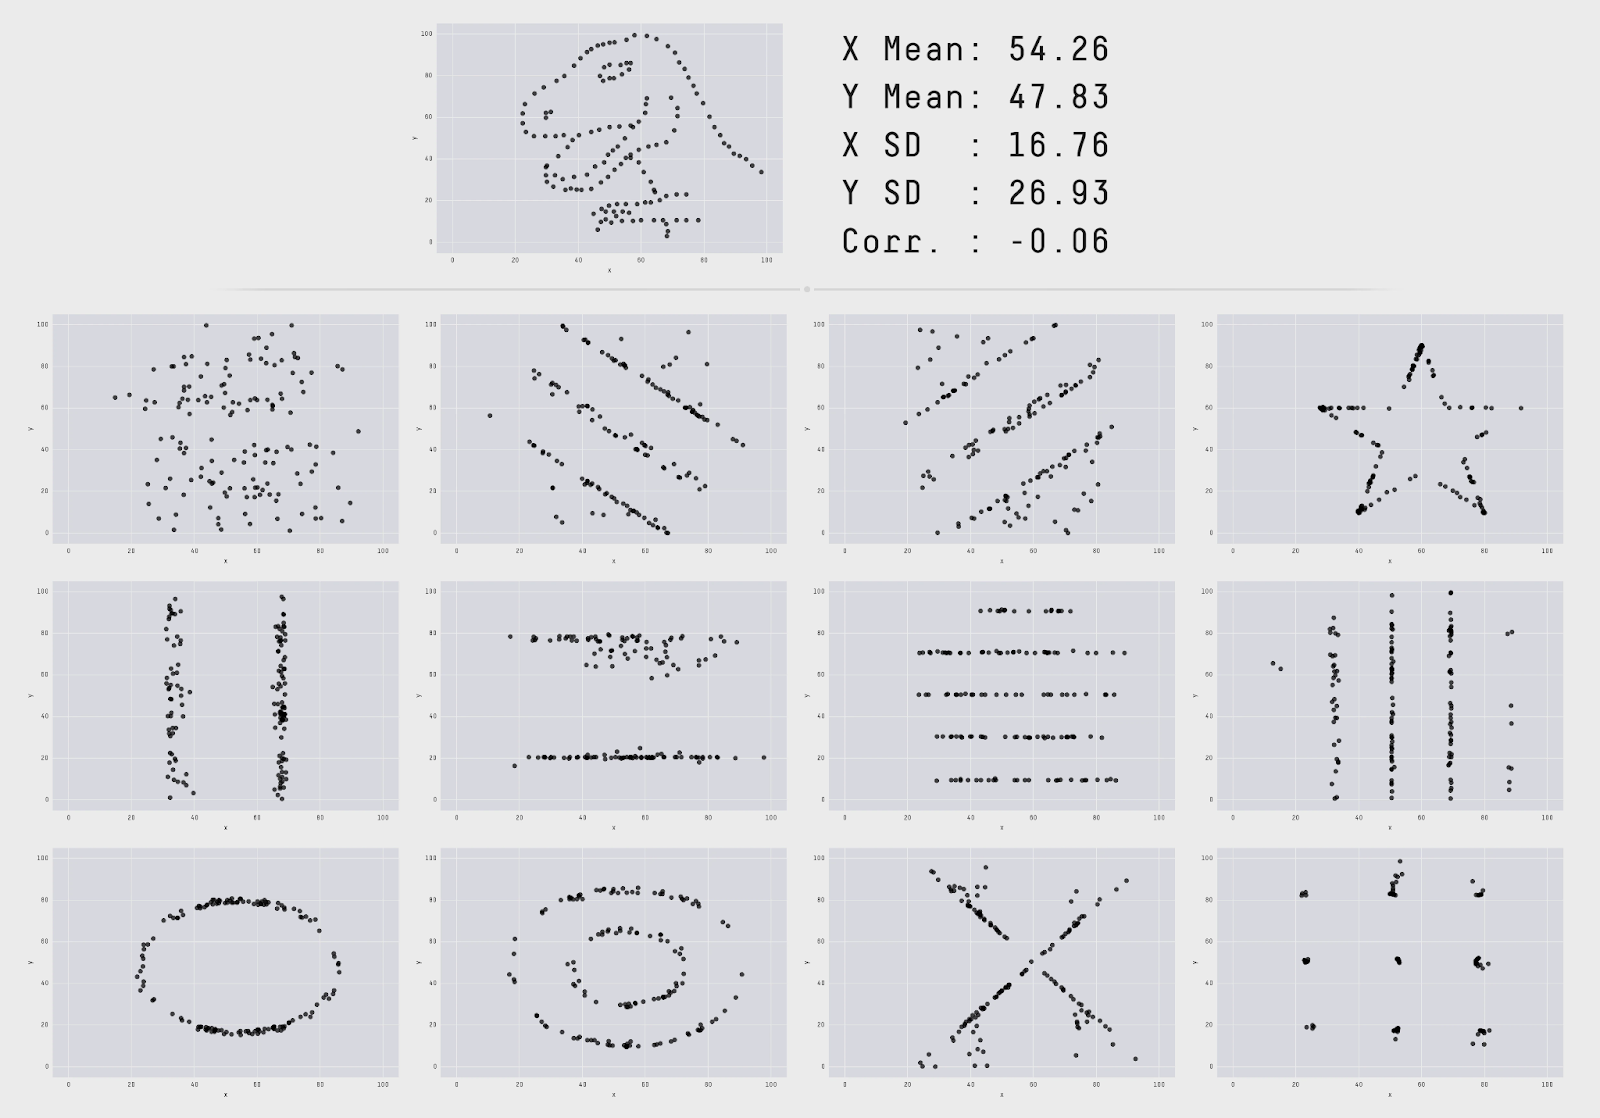
\includegraphics[width=\paperwidth]{figures/AllDinosGrey_1.png}}
\end{frame}
}

\begin{frame}
  \frametitle{Datasaurus}
  \href{http://www.thefunctionalart.com/2016/08/download-datasaurus-never-trust-summary.html}{Alberto Cairo: the Datasaurus}

  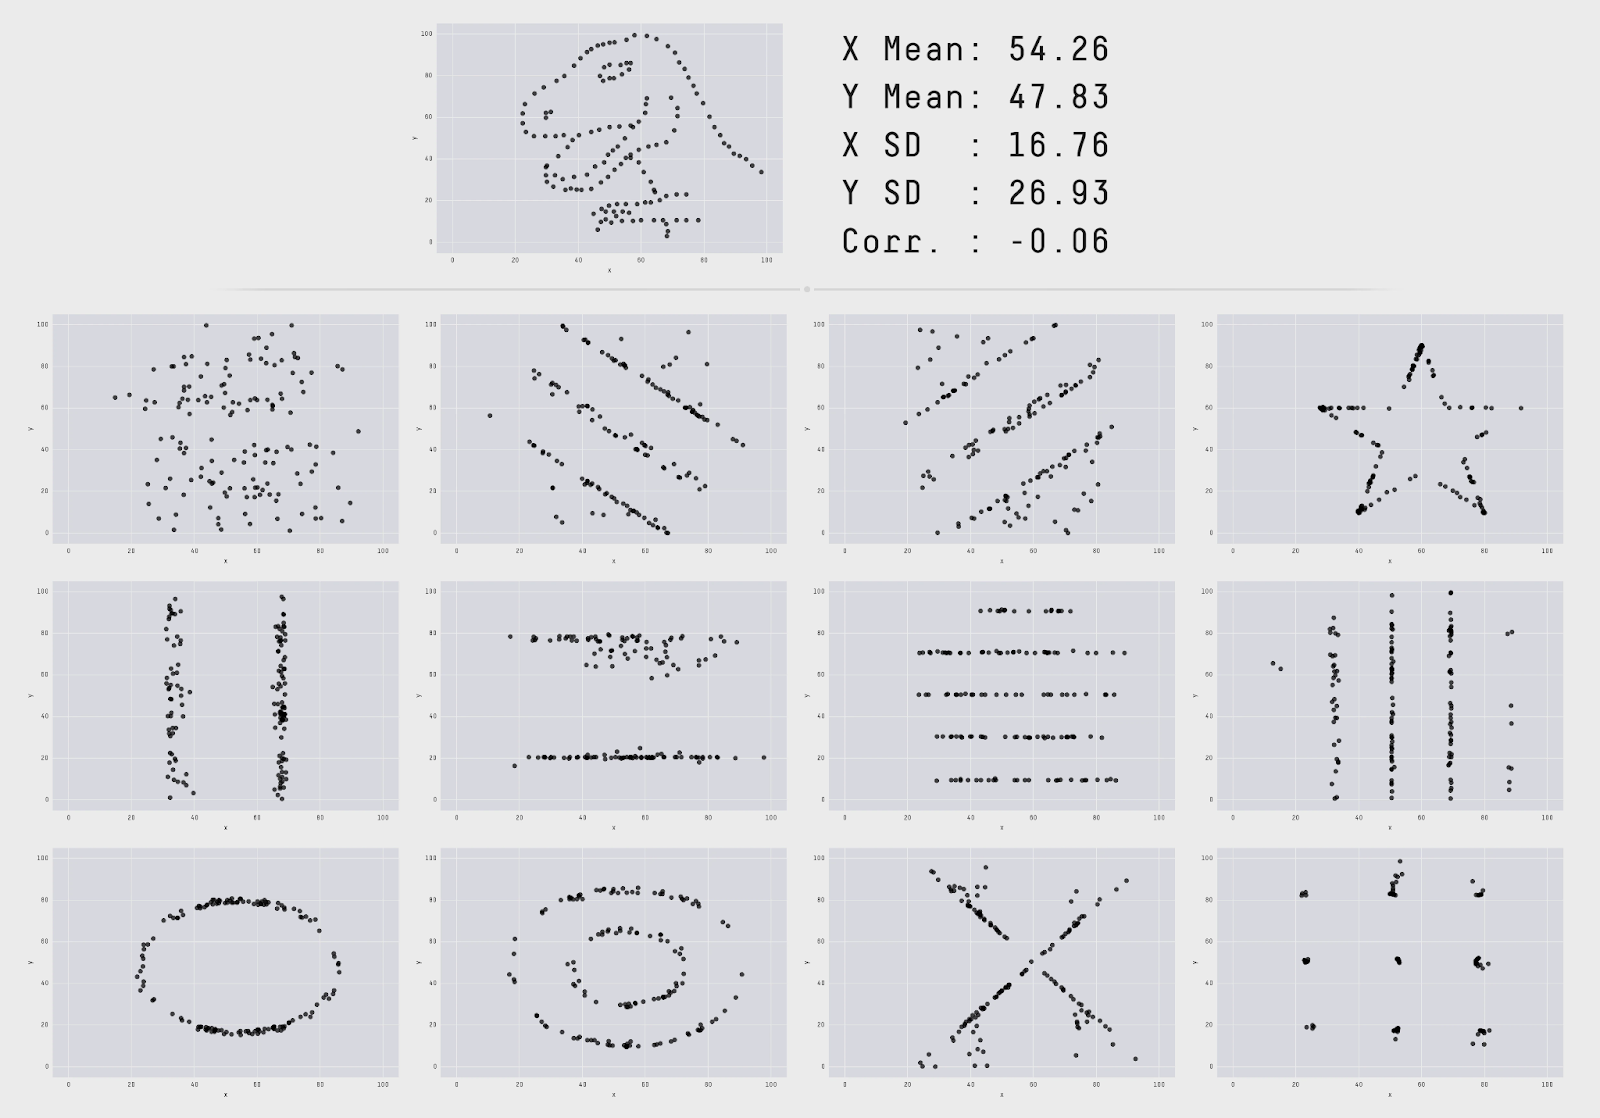
\includegraphics[width=7cm]{figures/AllDinosGrey_1.png}


\begin{quote}
Never trust summary statistics alone; always visualize your data
\end{quote}
\end{frame}

\begin{frame}
  \frametitle{Scatterplot}
  Eine Menge von Vektoren (Punkten) in $\mathbb{R}^2$ lässt sich darstellen, indem ein rechteckiger Ausschnitt des $\mathbb{R}^2$ auf die Plotfläche abgebildet wird und an jedem Punkt ein Symbol, etwa ein gefüllter Kreis, gezeichnet wird.

  \vspace{1cm}

  \texttt{scatter(x, y, marker='o')} in \texttt{matplotlib.pyplot}

  \vspace{1cm}

  Also z.B. wenn \texttt{data.shape == (N, 2)}, dann\\ \texttt{scatter(data[:, 0], data[:, 1])} \\
  um beide Spalten gegeneinander zu plotten.
\end{frame}

\begin{frame}
  \frametitle{Farbe im Scatterplot}
  Liegt zusätzlich zu $x$- und $y$-Werten noch eine dritte Variable vor, die sich in eine Farbskala umrechnen lässt, können wir diese nutzen.

  Ist z.B. \texttt{data.shape == (N, 3)} und das dritte Feature ist eine kategoriale Variable mit 3 möglichen Ausprägungen, so wird\\

  \texttt{scatter(data[:, 0], data[:, 1], c=data[:, 2])}

  die Punkte entsprechend einer Default-Colormap (cmap) mit 3 Farben unterschiedlich einfärben.
\end{frame}

\begin{frame}
  \frametitle{Linienplots}
  Unsere Plots von Funktionsgraphen waren Linienplots.
  Man kann auch einen Kreis als Linienplot darstellen, indem man entlang eines Kreises Punkte sampelt,
  etwa für einen \texttt{np.linspace} zwischen $0$ und $2\pi$ den Winkel:

  \vspace{1cm}

  \texttt{angles = np.linspace(0, 6.28, 360)}\\
  \texttt{plot(np.cos(angles), np.sin(angles), linewidth=2)}
  
\end{frame}


\begin{frame}
  \frametitle{Bar charts (Balkendiagramme)}
  Für nominal skalierte Merkmale: pro Ausprägung ein Rechteck (der Balken) fester Breite, dessen Höhe proportional zur Häufigkeit der Ausprägung in der Stichprobe ist.

  \vspace{1cm}

  \uncover<2->{
    Bei ordinal skalierten Features ist es sinnvoll, die Rechtecke entlang der $x$-Achse anzuordnen.
  }

  \vspace{1cm}

  \uncover<3->{
    \alert{Tortendiagramme} sind seltsam dargestellte Barcharts und in der Regel schlechter intuitiv zu erfassen als der entsprechende Barchart oder \alert{stacked Barchart} (gestapelt).
    }
  \end{frame}

  \begin{frame}
    \frametitle{Histogramme}
    Für Features mit unendlich vielen möglichen Ausprägungen, typischerweise auf Intervallskalen,
    ist ein Barchart nicht direkt sinnvoll.

    \vspace{1cm}

    Wir unterteilen die Skala in endlich viele Intervalle und bilden eine neue Variable: die Häufigkeit von Instanzen mit Ausprägung innerhalb des Intervalls. Diese neue Variable ist diskret, ihr Barchart heisst \alert{Histogramm} von der ursprünglichen Variable. Die Unterteilung in Intervalle heißt \alert{Binning}, die Größe eines Intervalls \alert{binsize (Eimergröße)}.

    \vspace{0.5cm}
    
    \href{https://www.atlassian.com/data/charts/histogram-complete-guide}{Empfehlung: Mike Yi: A complete guide to histograms}
  \end{frame}

  \begin{frame}
    \frametitle{Weitere Visualisierungen}
    \begin{itemize}[<+->]
      \item Boxplot (Box-and-Whiskers) zur Darstellung von Quantilen
      \item Violinenplot zur Darstellung einer Dichte im Boxplot
      \item Kartendarstellungen (etwa zweidimensionales Histogramm mit Farbe)
    \end{itemize}
  \end{frame}

\begin{frame}[separator]
  \frametitle{Die Grammatik der Grafiken}
\end{frame}

\begin{frame}
  \frametitle{Geschichte}
  \begin{itemize}
  \item 1983: Bertin: Semiology of Graphics
  \item 2000: Wilkinson, Anand, Grossman: The Grammar of Graphics
  \item 2005: Wickham: \texttt{ggplot2} R Paket
  \item 2010: Wickham: A Layered Grammar of Graphics
  \end{itemize}
\end{frame}

\begin{frame}
  \frametitle{Grammatik}
  \begin{itemize}
  \item Daten – Welche sollen visualisiert werden?
  \item Ästhetik – Achsen, Dimensionen
  \item Skalen – Werte skalieren? Nominal/Ordinal?
  \item Geometrie – Punkte, Linien, Polygone
  \item Statistik – z.B. Mittelwerte
  \item Facetten – Subplots
  \item Koordinatensysteme – kartesisch oder polar oder logarithmisch
  \end{itemize}
\end{frame}

\begin{frame}
  \frametitle{Schichten (Layer)}
  Eine Schicht besteht aus
  \begin{itemize}
\item Daten und ästhetische Zuordnungen (aes)
\item Statistischen Transformationen (stat)
\item Geometrischen Objekten (geom)
\item Positionsbestimmungen
\end{itemize}
\end{frame}

\begin{frame}
  \frametitle{Statistische Transformationen}
  Die wichtigsten statistischen Transformationen, die in ggplot2 implementiert sind, haben wir teilweise schon kennen gelernt:
  \begin{itemize}
\item bin: Teile stetigen Bereich in Bins (Klassen) und zähle Punkte in jeder Klasse.
\item boxplot: Berechne Statistik für Boxplot
\item contour: Berechne Konturlinien
\item density: Berechne eindimensionale Dichteschätzung
\item identity: Identitätsabbildung, $f(x) = x$
\item jitter: Verändere jeden Wert mit einem kleinen Zufallswert
\item smooth: Geglätteter Mittelwert von y, gegeben x
\item summary: Summierte Werte von y für jedes x
\item unique: Entferne Duplikate
\end{itemize}
\end{frame}

\begin{frame}
  \frametitle{Skalen}
Eine Skala im Sinne der Grammatik der Grafiken kontrolliert die Zuordnung von Daten zu den ästhetischen Attributen.

\vspace{0.3cm}

\uncover<2->{
Beispiel: eine reelle Variable zwischen $0$ und $1$
 lässt sich als Farbänderung von Blau zu Rot darstellen. Die Skala ist die Zuordnung aller Werte von $[0,1]$
 auf Farbwerte. Die Umkehrfunktion dieser Zuordnung lässt sich zur Darstellung einer Legende nutzen.
}

\vspace{0.3cm}

\uncover<3->{
  Beispiel: eine kategoriale Variable (etwa die Spezies im Iris-Datensatz) wird mit verschiedenen Symbolen dargestellt (etwa in einem Scatterplot). Die Zuordnung Ausprägung zu Symbol ist die Skala.
}
\end{frame}


\begin{frame}
  \frametitle{Farben}
  Bei der Wahl von Farben zur Visualisierung sollte man stets bedenken, dass schlechte Lichtverhältnisse bereits zu verminderter Farbwahrnehmung führen und daher Farbe möglichst nicht allein verwendet werden sollte - mindestens die Helligkeit sollte bereits ausreichen (früher: Druck in Graustufen). Auch ergänzt mit Linienstil (-dicke, gestrichelt, gepunktet) oder Symbolen (Kreise, Kreuze) wirkt Farbe.

  \vspace{1cm}

  \uncover<2->{
    Etwa jeder 12. Mann und jede 200. Frau können Farben nicht so unterscheiden wie die Mehrheit. Das ist so häufig, dass man Farbskalen verwenden sollte, die diese Menschen auch unterscheiden können.
    }
\end{frame}

{
\setbeamertemplate{navigation symbols}{}
\begin{frame}[plain]
  \vspace{-1cm}
    \makebox[\linewidth]{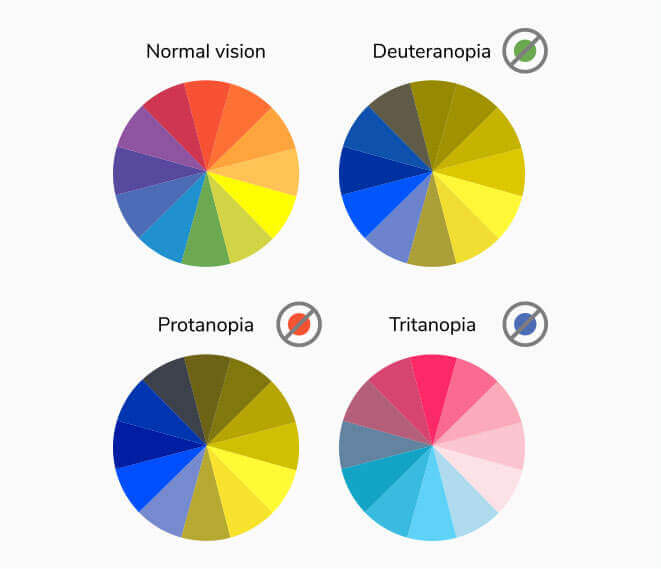
\includegraphics[height=\paperheight]{figures/color-blind-friendly-palette-13.jpg}}
\end{frame}
}

\begin{frame}
  \frametitle{Zusammenfassung}
  \begin{itemize}[<+->]
  \item Sie können Daten in verschiedene Skalenniveaus einteilen,
  \item anhand dessen deskriptive Statistiken (Häufigkeiten, Summen, Lagemaße zentraler Tendenz, Dispersionsmaße) berechnen,
  \item geeignete Visualisierungen auswählen (statistische Transformationen, Geometrien),
  \item mit Wahrscheinlichkeitsverteilungen modellieren und die Modelle visualisieren.
  \end{itemize}
\end{frame}

\begin{frame}
  \frametitle{Explorative Datenanalyse}
  In der EDA geht es darum, sich iterativ Daten zu erschließen und die Erkenntnisse zu kommunizieren.
  Dabei werden wiederholt diese Schritte durchgeführt:
  \begin{itemize}[<+->]
  \item Forschungsfragen formulieren (welche Skalen, Verteilungen, Zusammenhänge?)
  \item Daten visualisieren (deskriptive Statistik)
  \item Daten putzen (ggf. Ausreißer entfernen, Fehlstellen imputieren/interpolieren)
  \item Daten transformieren (Teile auswählen, neue Features generieren)
  \item Daten modellieren (statistische Modelle wählen, fitten)
  \end{itemize}
  Das werden wir noch üben!
\end{frame}

\begin{frame}[separator]
  \frametitle{Vielen Dank für Ihre Aufmerksamkeit!}
\end{frame}

\end{document}

%%% Local Variables:
%%% mode: latex
%%% TeX-master: t
%%% End:
